\section{The simulated neuron}

The simulated neuron used in this system tries to capture, through a time-stepped simulation, the functional essence of a biological neuron. A neuron receives input potentials $q_i$ (between -1 and 1) from the output of several other neurons, over time. The neuron sums up these potentials, at every time-step, and if the sum exceeds a threshold $Q_{th}$ it fires an activation potential that is then communicated via synapses to other neurons. After firing, the neuron's own potential drops to a small value below the baseline of 0 and then decays back to 0 by a factor of $k_p$ at every time-step. This decay constant for the potential, $k_p$, is always applied on the neuron and causes the potential to decay back to 0 even if the threshold has not been met and the neuron not been fired. Fig.~\ref{fig:c_potential_time} shows the potential of a single neuron that has been fired (red) and one that has not been fired (blue).

\begin{figure}[thp]
\centering
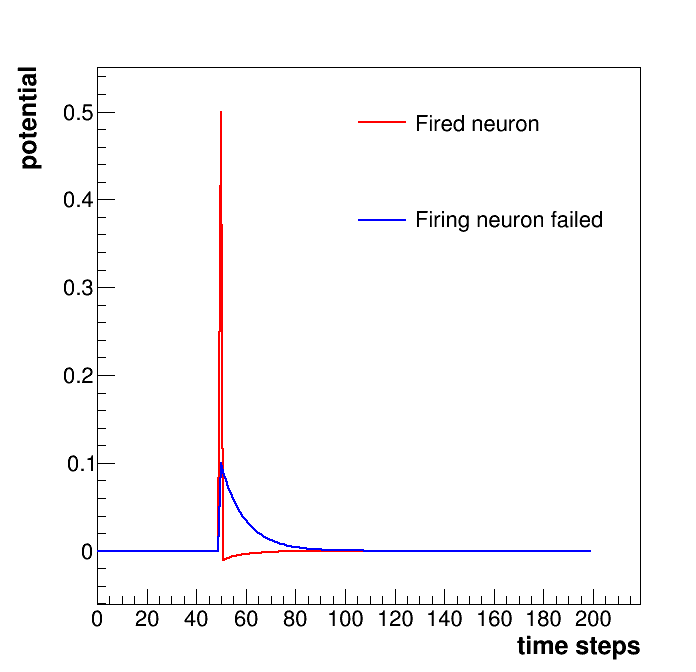
\includegraphics[width=0.6\textwidth]{c_potential_time.png}
\caption{The potential of a single neuron is plotted as a function of time. The red curve is for a neuron that is stimulated with a potential greater than the threshold $Q_{th}$ = 0.4 at time 50. It fires on its output and then drops its potential to -0.01. Thereafter, the potential decays by a factor of $k_p$ = 0.9 every time-step back to 0. In blue is the same neuron stimulated with a potential less than $Q_{th}$. It does not fire and the potential simply decays by $k_p$ back to 0.}
\label{fig:c_potential_time}
\end{figure}

\subsection{Output frequency from input frequency}

We can derive the frequency at which the neuron will fire if it is stimulated with a potential of $q$ applied every $t$ time-steps, i.e. with a frequency of $f_{in} = 1/t$. Since the potential will decay by a factor of $k_p$ at every time-step, the potential will reach $Q_{th}$ after $n$ time steps where:

\begin{equation*}
q(1 + k_p^t + k_p^{2t} ... + k_p^{nt}) = Q_{th}
\end{equation*}  

This is the sum of a geometric series, and we can write it in closed form as Eq.~\ref{eq:neuron:eq1}.

\begin{equation}
\label{eq:neuron:eq1}
\frac{Q_{th}}{q} = \frac{1-k^{t(n+1)}}{1-k^t}
\end{equation}

This can be solved for $n$ to derive the output frequency of the neuron $f_{out} = 1/nt$. The solution for $n$ is written in Eq.~\ref{eq:neuron:n}.

\begin{equation}
\label{eq:neuron:n}
n = \frac{\log(1-\frac{Q_{th}}{q}(1-k^t))}{t\log(k)}-1
\end{equation}

For this to be true, i.e. for the total potential to ever reach $Q_{th}$, the argument of the logarithm in the numerator has to be positive. This implies a minimum frequency of input firing given by Eq.~\ref{eq:neuron:fin}. If this condition is not met, the neuron does not reach the firing threshold as shown by the blue curve in Fig.~\ref{fig:c_potential_time_sawtooth}a. When the condition is met, the neuron repeatedly fires in intervals of $nt$ given by Eq.~\ref{eq:neuron:n} as shown by the red curve in Fig.~\ref{fig:c_potential_time_sawtooth}b.

\begin{equation}
\label{eq:neuron:fin}
\frac{1}{t} = f_{in} > \frac{\log(1-q/Q_{th})}{\log(k)}
\end{equation}

\begin{figure}[thp]
\centering
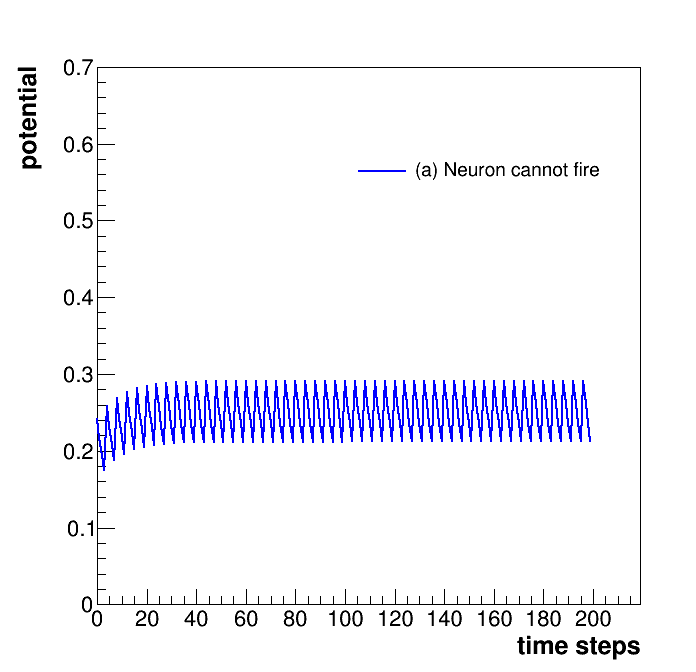
\includegraphics[width=0.49\textwidth]{c_potential_time_sawtooth_a.png}
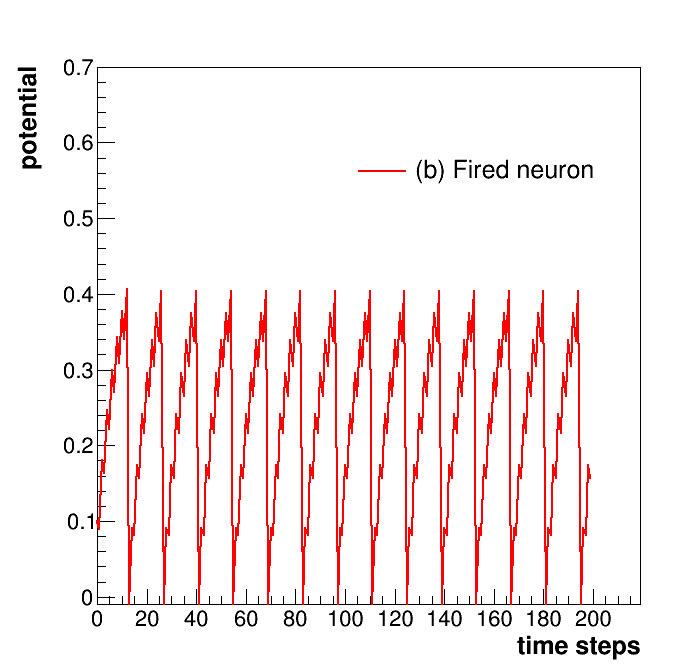
\includegraphics[width=0.49\textwidth]{c_potential_time_sawtooth_b.png}
\caption{(a) }
\label{fig:c_potential_time_sawtooth}
\end{figure}
